\documentclass[]{article}
\usepackage{lmodern}
\usepackage{amssymb,amsmath}
\usepackage{ifxetex,ifluatex}
\usepackage{fixltx2e} % provides \textsubscript
\ifnum 0\ifxetex 1\fi\ifluatex 1\fi=0 % if pdftex
  \usepackage[T1]{fontenc}
  \usepackage[utf8]{inputenc}
\else % if luatex or xelatex
  \ifxetex
    \usepackage{mathspec}
  \else
    \usepackage{fontspec}
  \fi
  \defaultfontfeatures{Ligatures=TeX,Scale=MatchLowercase}
\fi
% use upquote if available, for straight quotes in verbatim environments
\IfFileExists{upquote.sty}{\usepackage{upquote}}{}
% use microtype if available
\IfFileExists{microtype.sty}{%
\usepackage{microtype}
\UseMicrotypeSet[protrusion]{basicmath} % disable protrusion for tt fonts
}{}
\usepackage[margin=1in]{geometry}
\usepackage{hyperref}
\hypersetup{unicode=true,
            pdftitle={Transparancy for hydrocarbons use case},
            pdfborder={0 0 0},
            breaklinks=true}
\urlstyle{same}  % don't use monospace font for urls
\usepackage{color}
\usepackage{fancyvrb}
\newcommand{\VerbBar}{|}
\newcommand{\VERB}{\Verb[commandchars=\\\{\}]}
\DefineVerbatimEnvironment{Highlighting}{Verbatim}{commandchars=\\\{\}}
% Add ',fontsize=\small' for more characters per line
\usepackage{framed}
\definecolor{shadecolor}{RGB}{248,248,248}
\newenvironment{Shaded}{\begin{snugshade}}{\end{snugshade}}
\newcommand{\AlertTok}[1]{\textcolor[rgb]{0.94,0.16,0.16}{#1}}
\newcommand{\AnnotationTok}[1]{\textcolor[rgb]{0.56,0.35,0.01}{\textbf{\textit{#1}}}}
\newcommand{\AttributeTok}[1]{\textcolor[rgb]{0.77,0.63,0.00}{#1}}
\newcommand{\BaseNTok}[1]{\textcolor[rgb]{0.00,0.00,0.81}{#1}}
\newcommand{\BuiltInTok}[1]{#1}
\newcommand{\CharTok}[1]{\textcolor[rgb]{0.31,0.60,0.02}{#1}}
\newcommand{\CommentTok}[1]{\textcolor[rgb]{0.56,0.35,0.01}{\textit{#1}}}
\newcommand{\CommentVarTok}[1]{\textcolor[rgb]{0.56,0.35,0.01}{\textbf{\textit{#1}}}}
\newcommand{\ConstantTok}[1]{\textcolor[rgb]{0.00,0.00,0.00}{#1}}
\newcommand{\ControlFlowTok}[1]{\textcolor[rgb]{0.13,0.29,0.53}{\textbf{#1}}}
\newcommand{\DataTypeTok}[1]{\textcolor[rgb]{0.13,0.29,0.53}{#1}}
\newcommand{\DecValTok}[1]{\textcolor[rgb]{0.00,0.00,0.81}{#1}}
\newcommand{\DocumentationTok}[1]{\textcolor[rgb]{0.56,0.35,0.01}{\textbf{\textit{#1}}}}
\newcommand{\ErrorTok}[1]{\textcolor[rgb]{0.64,0.00,0.00}{\textbf{#1}}}
\newcommand{\ExtensionTok}[1]{#1}
\newcommand{\FloatTok}[1]{\textcolor[rgb]{0.00,0.00,0.81}{#1}}
\newcommand{\FunctionTok}[1]{\textcolor[rgb]{0.00,0.00,0.00}{#1}}
\newcommand{\ImportTok}[1]{#1}
\newcommand{\InformationTok}[1]{\textcolor[rgb]{0.56,0.35,0.01}{\textbf{\textit{#1}}}}
\newcommand{\KeywordTok}[1]{\textcolor[rgb]{0.13,0.29,0.53}{\textbf{#1}}}
\newcommand{\NormalTok}[1]{#1}
\newcommand{\OperatorTok}[1]{\textcolor[rgb]{0.81,0.36,0.00}{\textbf{#1}}}
\newcommand{\OtherTok}[1]{\textcolor[rgb]{0.56,0.35,0.01}{#1}}
\newcommand{\PreprocessorTok}[1]{\textcolor[rgb]{0.56,0.35,0.01}{\textit{#1}}}
\newcommand{\RegionMarkerTok}[1]{#1}
\newcommand{\SpecialCharTok}[1]{\textcolor[rgb]{0.00,0.00,0.00}{#1}}
\newcommand{\SpecialStringTok}[1]{\textcolor[rgb]{0.31,0.60,0.02}{#1}}
\newcommand{\StringTok}[1]{\textcolor[rgb]{0.31,0.60,0.02}{#1}}
\newcommand{\VariableTok}[1]{\textcolor[rgb]{0.00,0.00,0.00}{#1}}
\newcommand{\VerbatimStringTok}[1]{\textcolor[rgb]{0.31,0.60,0.02}{#1}}
\newcommand{\WarningTok}[1]{\textcolor[rgb]{0.56,0.35,0.01}{\textbf{\textit{#1}}}}
\usepackage{graphicx,grffile}
\makeatletter
\def\maxwidth{\ifdim\Gin@nat@width>\linewidth\linewidth\else\Gin@nat@width\fi}
\def\maxheight{\ifdim\Gin@nat@height>\textheight\textheight\else\Gin@nat@height\fi}
\makeatother
% Scale images if necessary, so that they will not overflow the page
% margins by default, and it is still possible to overwrite the defaults
% using explicit options in \includegraphics[width, height, ...]{}
\setkeys{Gin}{width=\maxwidth,height=\maxheight,keepaspectratio}
\IfFileExists{parskip.sty}{%
\usepackage{parskip}
}{% else
\setlength{\parindent}{0pt}
\setlength{\parskip}{6pt plus 2pt minus 1pt}
}
\setlength{\emergencystretch}{3em}  % prevent overfull lines
\providecommand{\tightlist}{%
  \setlength{\itemsep}{0pt}\setlength{\parskip}{0pt}}
\setcounter{secnumdepth}{0}
% Redefines (sub)paragraphs to behave more like sections
\ifx\paragraph\undefined\else
\let\oldparagraph\paragraph
\renewcommand{\paragraph}[1]{\oldparagraph{#1}\mbox{}}
\fi
\ifx\subparagraph\undefined\else
\let\oldsubparagraph\subparagraph
\renewcommand{\subparagraph}[1]{\oldsubparagraph{#1}\mbox{}}
\fi

%%% Use protect on footnotes to avoid problems with footnotes in titles
\let\rmarkdownfootnote\footnote%
\def\footnote{\protect\rmarkdownfootnote}

%%% Change title format to be more compact
\usepackage{titling}

% Create subtitle command for use in maketitle
\newcommand{\subtitle}[1]{
  \posttitle{
    \begin{center}\large#1\end{center}
    }
}

\setlength{\droptitle}{-2em}

  \title{Transparancy for hydrocarbons use case}
    \pretitle{\vspace{\droptitle}\centering\huge}
  \posttitle{\par}
    \author{}
    \preauthor{}\postauthor{}
    \date{}
    \predate{}\postdate{}
  

\begin{document}
\maketitle

\begin{itemize}
\tightlist
\item
  \#\#\#Retrieve provenance information from the package (Option 1)
\end{itemize}

\begin{Shaded}
\begin{Highlighting}[]
\KeywordTok{library}\NormalTok{(dataone)}
\KeywordTok{library}\NormalTok{(datapack)}
\end{Highlighting}
\end{Shaded}

\begin{verbatim}
## 
## Attaching package: 'datapack'
\end{verbatim}

\begin{verbatim}
## The following object is masked from 'package:raster':
## 
##     getData
\end{verbatim}

\begin{Shaded}
\begin{Highlighting}[]
\NormalTok{d1c <-}\StringTok{ }\KeywordTok{D1Client}\NormalTok{(}\StringTok{"PROD"}\NormalTok{, }\StringTok{"urn:node:GOA"}\NormalTok{)}
\NormalTok{pkg <-}\StringTok{ }\KeywordTok{getDataPackage}\NormalTok{(d1c, }\DataTypeTok{identifier =} \StringTok{"urn:uuid:1d23e155-3ef5-47c6-9612-027c80855e8d"}\NormalTok{, }\DataTypeTok{lazyLoad=}\OtherTok{TRUE}\NormalTok{, }\DataTypeTok{limit=}\StringTok{"0MB"}\NormalTok{, }\DataTypeTok{quiet=}\OtherTok{FALSE}\NormalTok{)}
\end{Highlighting}
\end{Shaded}

\begin{verbatim}
## Downloading package members for package with metadata identifier: urn:uuid:3249ada0-afe3-4dd6-875e-0f7928a4c171
## Downloaded object at URL https://goa.nceas.ucsb.edu/goa/d1/mn/v2/object/urn:uuid:3249ada0-afe3-4dd6-875e-0f7928a4c171
## Lazy Loaded object at URL https://goa.nceas.ucsb.edu/goa/d1/mn/v2/object/urn:uuid:b4b3cc45-4953-43d3-910a-847528577531
## Lazy Loaded object at URL https://goa.nceas.ucsb.edu/goa/d1/mn/v2/object/urn:uuid:44108e76-405d-4d58-b1b3-fb4b55e3fff9
## Lazy Loaded object at URL https://goa.nceas.ucsb.edu/goa/d1/mn/v2/object/urn:uuid:66c416af-84e6-4c7e-92a9-4413cf8acd7b
## Lazy Loaded object at URL https://goa.nceas.ucsb.edu/goa/d1/mn/v2/object/urn:uuid:c2f47e88-cc2b-47db-a105-101b80e80334
## Skipping metadata object, already downloaded
## Lazy Loaded object at URL https://goa.nceas.ucsb.edu/goa/d1/mn/v2/object/urn:uuid:780a5cff-6071-47d1-a52f-8f7a60c24625
## Lazy Loaded object at URL https://goa.nceas.ucsb.edu/goa/d1/mn/v2/object/urn:uuid:9490ce50-b7bc-4fe8-89d1-5b00736df835
## Lazy Loaded object at URL https://goa.nceas.ucsb.edu/goa/d1/mn/v2/object/urn:uuid:ae595730-172a-43d0-91f8-3173663d7dce
## Lazy Loaded object at URL https://goa.nceas.ucsb.edu/goa/d1/mn/v2/object/urn:uuid:5cde46ff-2e8e-4f40-97a1-eb4c4851f22f
## Lazy Loaded object at URL https://goa.nceas.ucsb.edu/goa/d1/mn/v2/object/urn:uuid:a8ed4776-1e17-426f-9f54-98073ae35b5f
## Lazy Loaded object at URL https://goa.nceas.ucsb.edu/goa/d1/mn/v2/object/urn:uuid:d31ea97c-e061-43f8-af06-62664671f166
## Lazy Loaded object at URL https://goa.nceas.ucsb.edu/goa/d1/mn/v2/object/urn:uuid:5f57c5d3-65f2-4d46-83f5-67f8104c62dd
## Getting resource map with id: urn:uuid:1d23e155-3ef5-47c6-9612-027c80855e8d
\end{verbatim}

\begin{Shaded}
\begin{Highlighting}[]
\NormalTok{saveWidth <-}\StringTok{ }\KeywordTok{getOption}\NormalTok{(}\StringTok{"width"}\NormalTok{)}
\KeywordTok{options}\NormalTok{(}\DataTypeTok{width=}\DecValTok{150}\NormalTok{)}
\NormalTok{pkg}
\end{Highlighting}
\end{Shaded}

\begin{verbatim}
## Members:
## 
## filename                                       format                mediaType  size     identifier                                    modified local 
## metadata.xml                                   eml://eco...eml-2.1.1 NA         142895   urn:uuid:3249ada0-afe3-4dd6-875e-0f7928a4c171 n        y     
## Total_Aromatic_Alkanes_PWS.csv                 text/csv              NA         2801033  urn:uuid:44108e76-405d-4d58-b1b3-fb4b55e3fff9 n        n     
## PAH.csv                                        text/csv              NA         5525560  urn:uuid:5cde46ff-2e8e-4f40-97a1-eb4c4851f22f n        n     
## Sample.csv                                     text/csv              NA         1500015  urn:uuid:5f57c5d3-65f2-4d46-83f5-67f8104c62dd n        n     
## CollectionMethods.csv                          text/csv              NA         793      urn:uuid:66c416af-84e6-4c7e-92a9-4413cf8acd7b n        n     
## hcdbSamplesGOA.png                             image/png             NA         58073    urn:uuid:780a5cff-6071-47d1-a52f-8f7a60c24625 n        n     
## hcdbSites.R                                    application/R         tex...rsrc 3005     urn:uuid:9490ce50-b7bc-4fe8-89d1-5b00736df835 n        n     
## Total_PAH_and_Alkanes_GoA_Hydrocarbons_Clean.R application/R         tex...rsrc 5080     urn:uuid:a8ed4776-1e17-426f-9f54-98073ae35b5f n        n     
## Non-EVOS_SINs.csv                              text/csv              NA         3545     urn:uuid:ae595730-172a-43d0-91f8-3173663d7dce n        n     
## hcdbSampleLocs.png                             image/png             NA         101868   urn:uuid:b4b3cc45-4953-43d3-910a-847528577531 n        n     
## DataDownload.R                                 application/R         tex...rsrc 1847     urn:uuid:c2f47e88-cc2b-47db-a105-101b80e80334 n        n     
## Alkane.csv                                     text/csv              NA         3932743  urn:uuid:d31ea97c-e061-43f8-af06-62664671f166 n        n     
## 
## Package identifier: urn:uuid:1d23e155-3ef5-47c6-9612-027c80855e8d
## RightsHolder: http://orcid.org/0000-0002-1006-9496
## 
## 
## Relationships:
##                                           subject                 predicate                                         object
## 64                           _r1529524071r58792r2                  rdf:type                               prov:Association
## 40                           _r1529524071r58792r2              prov:hadPlan                                 DataDownload.R
## 47                           _r1529524071r58792r3                  rdf:type                               prov:Association
## 51                           _r1529524071r58792r3              prov:hadPlan Total_PAH_and_Alkanes_GoA_Hydrocarbons_Clean.R
## 60                           _r1529524071r58792r4                  rdf:type                               prov:Association
## 54                           _r1529524071r58792r4              prov:hadPlan                                    hcdbSites.R
## 65                                     Alkane.csv       cito:isDocumentedBy                                   metadata.xml
## 49                                     Alkane.csv                  rdf:type                                   provone:Data
## 24                                     Alkane.csv       prov:wasGeneratedBy  urn:uuid:e4e1e40a-58bb-497e-af9a-18a2807d7444
## 8                           CollectionMethods.csv       cito:isDocumentedBy                                   metadata.xml
## 53                          CollectionMethods.csv                  rdf:type                                   provone:Data
## 14                          CollectionMethods.csv       prov:wasGeneratedBy  urn:uuid:e4e1e40a-58bb-497e-af9a-18a2807d7444
## 7                                  DataDownload.R       cito:isDocumentedBy                                   metadata.xml
## 62                                 DataDownload.R                  rdf:type                                provone:Program
## 55                             hcdbSampleLocs.png       cito:isDocumentedBy                                   metadata.xml
## 63                             hcdbSampleLocs.png                  rdf:type                                   provone:Data
## 13                             hcdbSampleLocs.png       prov:wasDerivedFrom                 Total_Aromatic_Alkanes_PWS.csv
## 2                              hcdbSampleLocs.png       prov:wasGeneratedBy  urn:uuid:d248eca5-064f-4ee4-8c8c-59838fa94666
## 20                             hcdbSamplesGOA.png       cito:isDocumentedBy                                   metadata.xml
## 52                             hcdbSamplesGOA.png                  rdf:type                                   provone:Data
## 4                              hcdbSamplesGOA.png       prov:wasDerivedFrom                 Total_Aromatic_Alkanes_PWS.csv
## 68                             hcdbSamplesGOA.png       prov:wasGeneratedBy  urn:uuid:d248eca5-064f-4ee4-8c8c-59838fa94666
## 3                                     hcdbSites.R       cito:isDocumentedBy                                   metadata.xml
## 22                                    hcdbSites.R                  rdf:type                                provone:Program
## 25                                   metadata.xml            cito:documents                                   metadata.xml
## 26                                   metadata.xml            cito:documents                 Total_Aromatic_Alkanes_PWS.csv
## 27                                   metadata.xml            cito:documents                                        PAH.csv
## 28                                   metadata.xml            cito:documents                                     Sample.csv
## 29                                   metadata.xml            cito:documents                          CollectionMethods.csv
## 30                                   metadata.xml            cito:documents                             hcdbSamplesGOA.png
## 31                                   metadata.xml            cito:documents                                    hcdbSites.R
## 32                                   metadata.xml            cito:documents Total_PAH_and_Alkanes_GoA_Hydrocarbons_Clean.R
## 33                                   metadata.xml            cito:documents                              Non-EVOS_SINs.csv
## 34                                   metadata.xml            cito:documents                             hcdbSampleLocs.png
## 35                                   metadata.xml            cito:documents                                 DataDownload.R
## 36                                   metadata.xml            cito:documents                                     Alkane.csv
## 10                                   metadata.xml       cito:isDocumentedBy                                   metadata.xml
## 46                              Non-EVOS_SINs.csv       cito:isDocumentedBy                                   metadata.xml
## 9                               Non-EVOS_SINs.csv                  rdf:type                                   provone:Data
## 11                                        PAH.csv       cito:isDocumentedBy                                   metadata.xml
## 12                                        PAH.csv                  rdf:type                                   provone:Data
## 59                                        PAH.csv       prov:wasGeneratedBy  urn:uuid:e4e1e40a-58bb-497e-af9a-18a2807d7444
## 67                                     Sample.csv       cito:isDocumentedBy                                   metadata.xml
## 15                                     Sample.csv                  rdf:type                                   provone:Data
## 39                                     Sample.csv       prov:wasGeneratedBy  urn:uuid:e4e1e40a-58bb-497e-af9a-18a2807d7444
## 41                 Total_Aromatic_Alkanes_PWS.csv       cito:isDocumentedBy                                   metadata.xml
## 48                 Total_Aromatic_Alkanes_PWS.csv                  rdf:type                                   provone:Data
## 16                 Total_Aromatic_Alkanes_PWS.csv       prov:wasDerivedFrom                                        PAH.csv
## 17                 Total_Aromatic_Alkanes_PWS.csv       prov:wasDerivedFrom                                     Sample.csv
## 18                 Total_Aromatic_Alkanes_PWS.csv       prov:wasDerivedFrom                              Non-EVOS_SINs.csv
## 19                 Total_Aromatic_Alkanes_PWS.csv       prov:wasDerivedFrom                                     Alkane.csv
## 1                  Total_Aromatic_Alkanes_PWS.csv       prov:wasGeneratedBy  urn:uuid:a4e3b687-fb17-4f37-a185-13d4d59d06f9
## 58 Total_PAH_and_Alkanes_GoA_Hydrocarbons_Clean.R       cito:isDocumentedBy                                   metadata.xml
## 6  Total_PAH_and_Alkanes_GoA_Hydrocarbons_Clean.R                  rdf:type                                provone:Program
## 57  urn:uuid:a4e3b687-fb17-4f37-a185-13d4d59d06f9        dcterms:identifier  urn:uuid:a4e3b687-fb17-4f37-a185-13d4d59d06f9
## 37  urn:uuid:a4e3b687-fb17-4f37-a185-13d4d59d06f9                  rdf:type                              provone:Execution
## 66  urn:uuid:a4e3b687-fb17-4f37-a185-13d4d59d06f9 prov:qualifiedAssociation                           _r1529524071r58792r3
## 42  urn:uuid:a4e3b687-fb17-4f37-a185-13d4d59d06f9                 prov:used                                        PAH.csv
## 43  urn:uuid:a4e3b687-fb17-4f37-a185-13d4d59d06f9                 prov:used                                     Sample.csv
## 44  urn:uuid:a4e3b687-fb17-4f37-a185-13d4d59d06f9                 prov:used                              Non-EVOS_SINs.csv
## 45  urn:uuid:a4e3b687-fb17-4f37-a185-13d4d59d06f9                 prov:used                                     Alkane.csv
## 21  urn:uuid:d248eca5-064f-4ee4-8c8c-59838fa94666        dcterms:identifier  urn:uuid:d248eca5-064f-4ee4-8c8c-59838fa94666
## 56  urn:uuid:d248eca5-064f-4ee4-8c8c-59838fa94666                  rdf:type                              provone:Execution
## 23  urn:uuid:d248eca5-064f-4ee4-8c8c-59838fa94666 prov:qualifiedAssociation                           _r1529524071r58792r4
## 38  urn:uuid:d248eca5-064f-4ee4-8c8c-59838fa94666                 prov:used                 Total_Aromatic_Alkanes_PWS.csv
## 61  urn:uuid:e4e1e40a-58bb-497e-af9a-18a2807d7444        dcterms:identifier  urn:uuid:e4e1e40a-58bb-497e-af9a-18a2807d7444
## 50  urn:uuid:e4e1e40a-58bb-497e-af9a-18a2807d7444                  rdf:type                              provone:Execution
## 5   urn:uuid:e4e1e40a-58bb-497e-af9a-18a2807d7444 prov:qualifiedAssociation                           _r1529524071r58792r2
\end{verbatim}

\begin{itemize}
\tightlist
\item
  \#\#\#Record provenance using recordr (Option2)
\end{itemize}

\begin{Shaded}
\begin{Highlighting}[]
\KeywordTok{source}\NormalTok{(}\StringTok{"./setup.R"}\NormalTok{)}
\end{Highlighting}
\end{Shaded}

\begin{verbatim}
## Checking rgeos availability: TRUE
\end{verbatim}

\begin{verbatim}
## rgeos version: 0.3-28, (SVN revision 572)
##  GEOS runtime version: 3.6.2-CAPI-1.10.2 4d2925d6 
##  Linking to sp version: 1.3-1 
##  Polygon checking: TRUE
\end{verbatim}

\begin{verbatim}
## rgdal: version: 1.3-2, (SVN revision 755)
##  Geospatial Data Abstraction Library extensions to R successfully loaded
##  Loaded GDAL runtime: GDAL 2.3.0, released 2018/05/04
##  Path to GDAL shared files: /usr/local/Cellar/gdal/2.3.0/share/gdal
##  GDAL binary built with GEOS: TRUE 
##  Loaded PROJ.4 runtime: Rel. 5.1.0, June 1st, 2018, [PJ_VERSION: 510]
##  Path to PROJ.4 shared files: (autodetected)
##  Linking to sp version: 1.3-1
\end{verbatim}

\begin{verbatim}
## -- Attaching packages ---------------------------------------------------------------------------------------------- tidyverse 1.2.1 --
\end{verbatim}

\begin{verbatim}
## √ ggplot2 2.2.1     √ purrr   0.2.4
## √ tibble  1.4.2     √ dplyr   0.7.4
## √ tidyr   0.8.1     √ stringr 1.2.0
## √ readr   1.1.1     √ forcats 0.3.0
\end{verbatim}

\begin{verbatim}
## -- Conflicts ------------------------------------------------------------------------------------------------- tidyverse_conflicts() --
## x tidyr::extract() masks raster::extract()
## x dplyr::filter()  masks stats::filter()
## x dplyr::lag()     masks stats::lag()
## x dplyr::select()  masks raster::select()
\end{verbatim}

\begin{Shaded}
\begin{Highlighting}[]
\KeywordTok{library}\NormalTok{(recordr)}
\NormalTok{rc <-}\StringTok{ }\KeywordTok{new}\NormalTok{(}\StringTok{"Recordr"}\NormalTok{)}
\end{Highlighting}
\end{Shaded}

\begin{verbatim}
## A new recordr home directory has been created at:
## 
##  /var/folders/7t/xdmtt00j0w53slb206w9xh100000gn/T//RtmpNY5TWl/recordr
\end{verbatim}

\begin{verbatim}
## The recordr package will save run information to this directory, which is under
\end{verbatim}

\begin{verbatim}
## the R session temporary directory. Therefore the information that recordr collects
\end{verbatim}

\begin{verbatim}
## will be removed by R when the current R session ends.
\end{verbatim}

\begin{verbatim}
## 
## If you wish to change the recordr home directory so that information is saved to a
\end{verbatim}

\begin{verbatim}
## permanent location please use the "newDir" argument, for example
\end{verbatim}

\begin{verbatim}
## 
##  "rc <- new("Recordr", newDir="/Users/bobsmith/recordr")
\end{verbatim}

\begin{Shaded}
\begin{Highlighting}[]
\KeywordTok{record}\NormalTok{(rc, }\StringTok{"./scripts/Total_PAH_and_Alkanes_GoA_Hydrocarbons_Clean.R"}\NormalTok{, }\DataTypeTok{tag=}\StringTok{"total_pah_and_alkanes_goa_hydrocarbons_clean script1"}\NormalTok{)}
\end{Highlighting}
\end{Shaded}

\begin{verbatim}
## 'data.frame':    16960 obs. of  72 variables:
##  $ Funding     : chr  "EVOSTC" "EVOSTC" "EVOSTC" "EVOSTC" ...
##  $ Sin         : int  -600 -600 -557 -557 -900 20120312 20120313 20120310 20120309 20120308 ...
##  $ type        : chr  "QC" "QC" "QC" "QC" ...
##  $ Rep         : int  1 2 1 2 1 1 1 1 1 1 ...
##  $ LAB         : chr  "ABL" "ABL" "ABL" "ABL" ...
##  $ QCbatch     : chr  "20120827MZ" "20120827MZ" "20120827MZ" "20120827MZ" ...
##  $ strMAT      : chr  "sed" "sed" "sed" "sed" ...
##  $ LabSam      : chr  "NISTARO" "NISTARO" "AREF" "BREF" ...
##  $ Vol         : int  NA NA NA NA NA NA NA NA NA NA ...
##  $ Proportion  : num  NA NA NA NA NA NA NA NA NA NA ...
##  $ DryWt       : num  1 1 0.00678 0.00678 1 ...
##  $ WetWt       : num  1 1 0.00678 0.00678 1 ...
##  $ AnalysisType: chr  "QCCALI" "QCCALI" "QCOIL" "QCOIL" ...
##  $ Catno       : chr  "RMB_000" "RMB_000" "RMB_000" "RMB_000" ...
##  $ NaphD8      : num  92.5 92.5 88.7 86.7 108.4 ...
##  $ Acend10     : num  100.6 101.1 94.5 94.2 116.1 ...
##  $ Phend10     : num  101.1 101 94.9 95.2 116.3 ...
##  $ Anthra10    : num  NA NA NA NA NA NA NA NA NA NA ...
##  $ Banth12     : num  NA NA NA NA NA NA NA NA NA NA ...
##  $ Chryd12     : num  104.5 104.8 94.6 93.5 114.3 ...
##  $ Benad12     : num  114 114 115 113 133 ...
##  $ Peryd12     : num  106.5 109.5 89.3 91.8 106.7 ...
##  $ Units       : chr  "ng/g" "ng/g" "ng/g oil" "ng/g oil" ...
##  $ Naph        : num  247 247 124275 136809 0 ...
##  $ Menap2      : num  180 181 477226 487966 0 ...
##  $ MENAP1      : num  160 161 341500 345107 0 ...
##  $ DIMETH      : num  138 137 501639 503703 0 ...
##  $ C2NAPH      : num  412 412 1784545 1737098 0 ...
##  $ TRIMETH     : num  0 0 237407 239645 0 ...
##  $ C3NAPH      : num  0 0 1602999 1701227 0 ...
##  $ C4NAPH      : num  0 0 961949 990175 0 ...
##  $ BIPHENYL    : num  114 114 23663 23529 111 ...
##  $ ACENTHY     : num  138 134 15476 0 0 ...
##  $ ACENTHE     : num  118 118 16798 16649 0 ...
##  $ FLUORENE    : num  106 107 32643 33024 0 ...
##  $ C1FLUOR     : num  0 0 111440 113162 0 ...
##  $ C2FLUOR     : num  0 0 179608 180330 0 ...
##  $ C3FLUOR     : num  0 0 209519 199383 0 ...
##  $ C4FLUOR     : num  0 0 25311 25879 0 ...
##  $ DITHIO      : num  96.1 96.8 48726.8 45625.9 0 ...
##  $ C1DITHIO    : num  0 0 181422 183124 0 ...
##  $ C2DITHIO    : num  0 0 293077 296922 0 ...
##  $ C3DITHIO    : num  0 0 258189 258230 0 ...
##  $ C4DITHIO    : num  0 0 36010 37554 0 ...
##  $ PHENANTH    : num  245 245 97646 99282 0 ...
##  $ MEPHEN1     : num  202 205 97291 97390 0 ...
##  $ C1PHENAN    : num  978 980 470442 477279 0 ...
##  $ C2PHENAN    : num  0 167 733661 734837 0 ...
##  $ C3PHENAN    : num  0 0 502830 539533 0 ...
##  $ C4PHENAN    : num  0 0 230727 228864 0 ...
##  $ ANTHRA      : num  83.7 84.1 3669.9 2878 0 ...
##  $ FLUORANT    : num  190 189 2667 2660 0 ...
##  $ PYRENE      : num  208 208 8622 8475 0 ...
##  $ C1FLUORA    : num  0 0 40463 38925 0 ...
##  $ C2FLUORA    : num  0 0 83041 87831 0 ...
##  $ C3FLUORA    : num  0 0 65452 59747 0 ...
##  $ C4FLUORA    : num  0 0 46432 45956 0 ...
##  $ BENANTH     : num  107 107 4676 3706 0 ...
##  $ CHRYSENE    : num  104 104 11122 11243 0 ...
##  $ C1CHRYS     : num  89 88.6 26538.6 28080.2 0 ...
##  $ C2CHRYS     : num  0 0 53113 47651 0 ...
##  $ C3CHRYS     : num  0 0 22029 21114 0 ...
##  $ C4CHRYS     : num  0 0 7310 8871 0 ...
##  $ BENZOBFL    : num  193 195 834 1026 0 ...
##  $ BENZOKFL    : num  74.5 74.7 130.6 136.6 0 ...
##  $ BENEPY      : num  108 109 2575 3014 0 ...
##  $ BENAPY      : num  112 113 632 883 0 ...
##  $ PERYLENE    : num  103 102 33971 33769 0 ...
##  $ INDENO      : num  117 113 0 0 0 ...
##  $ DIBENZ      : num  111 112 302 350 0 ...
##  $ BENZOP      : num  142 132 1335 1611 0 ...
##  $ comment     : logi  NA NA NA NA NA NA ...
\end{verbatim}

\begin{verbatim}
## ----------------------------------------------------------------------------------------------------------------------------------------------------
\end{verbatim}

\begin{verbatim}
## You have loaded plyr after dplyr - this is likely to cause problems.
## If you need functions from both plyr and dplyr, please load plyr first, then dplyr:
## library(plyr); library(dplyr)
\end{verbatim}

\begin{verbatim}
## ----------------------------------------------------------------------------------------------------------------------------------------------------
\end{verbatim}

\begin{verbatim}
## 
## Attaching package: 'plyr'
\end{verbatim}

\begin{verbatim}
## The following objects are masked from 'package:dplyr':
## 
##     arrange, count, desc, failwith, id, mutate, rename, summarise, summarize
\end{verbatim}

\begin{verbatim}
## The following object is masked from 'package:purrr':
## 
##     compact
\end{verbatim}

\begin{verbatim}
## 'data.frame':    15955 obs. of  53 variables:
##  $ Funding     : chr  "EVOSTC" "EVOSTC" "EVOSTC" "EVOSTC" ...
##  $ Sin         : int  -902 -902 -902 -902 -902 -902 -902 -902 -902 -902 ...
##  $ type        : chr  "QC" "QC" "QC" "QC" ...
##  $ Rep         : int  1 1 1 1 1 1 1 1 1 1 ...
##  $ LAB         : chr  "ABL" "ABL" "ABL" "ABL" ...
##  $ QCbatch     : chr  "W102390" "L012391" "W101090" "W100990" ...
##  $ strMAT      : chr  "" "" "" "" ...
##  $ LabSam      : chr  "" "" "" "" ...
##  $ Vol         : int  NA NA NA NA NA NA NA NA NA NA ...
##  $ Proportion  : logi  NA NA NA NA NA NA ...
##  $ DryWt       : num  NA NA NA NA NA NA NA NA NA NA ...
##  $ WetWt       : num  1 1 1 1 1 1 1 1 1 1 ...
##  $ AnalysisType: chr  "" "" "" "" ...
##  $ Catno       : chr  "NMFS_000" "NMFS_000" "NMFS_000" "NMFS_000" ...
##  $ C12d26      : num  15.4 40.9 44.4 52.3 56.3 ...
##  $ C16d34      : num  45.2 68.9 77.8 62.3 64.8 ...
##  $ C20d42      : num  79.7 88.6 89.2 79.9 79.1 ...
##  $ C24d50      : num  87.8 92.2 86.9 84.7 82 ...
##  $ C30d64      : num  88.3 96.2 86.1 84.3 70.1 ...
##  $ Units       : chr  "" "" "" "" ...
##  $ C9ALK       : num  0 0 0 0 0 0 0 0 0 0 ...
##  $ C10ALK      : num  5799 9024 9399 9067 9731 ...
##  $ C11ALK      : num  7115 9666 9279 9244 9789 ...
##  $ C12ALK      : num  10957 11305 10176 10265 10754 ...
##  $ C13ALK      : num  15396 12642 10918 10936 11227 ...
##  $ C14ALK      : num  6703 8743 7349 9347 9903 ...
##  $ C15ALK      : num  8123 9500 8664 9265 9797 ...
##  $ C16ALK      : num  11290 11966 10943 10940 11554 ...
##  $ C17ALK      : num  14662 13658 12383 12285 13160 ...
##  $ PRISTANE    : num  15357 14620 12439 12720 13234 ...
##  $ C18ALK      : num  10570 12613 12216 11400 12166 ...
##  $ PHYTANE     : num  51.9 83.7 10.6 31 99.4 ...
##  $ C19ALK      : num  10422 11554 10845 10516 11108 ...
##  $ C20ALK      : num  10096 10536 9709 9759 10198 ...
##  $ C21ALK      : num  10345 10350 9295 9685 10083 ...
##  $ C22ALK      : num  10735 11262 10937 10703 10884 ...
##  $ C23ALK      : num  9798 10094 9605 9596 9805 ...
##  $ C24ALK      : num  10298 10559 9773 9919 10220 ...
##  $ C25ALK      : num  9695 10025 9026 9288 9635 ...
##  $ C26ALK      : num  9627 10042 8828 9123 9512 ...
##  $ C27ALK      : num  4097 4298 3642 3791 4000 ...
##  $ C28ALK      : num  10516 10852 10689 10838 10926 ...
##  $ C29ALK      : num  9499 9863 9407 9448 9671 ...
##  $ C30ALK      : num  10179 10519 9718 9672 10053 ...
##  $ C31ALK      : num  0 0 0 0 0 0 0 0 0 0 ...
##  $ C32ALK      : num  10168 10027 9036 8612 8990 ...
##  $ C33ALK      : num  0 0 0 0 0 0 0 0 0 0 ...
##  $ C34ALK      : num  10776 10199 8883 8425 5148 ...
##  $ C35ALK      : num  0 0 0 0 0 0 0 0 0 0 ...
##  $ C36ALK      : num  0 0 0 0 0 0 0 0 0 0 ...
##  $ TOTALKANES  : num  242657 254894 233495 235218 241905 ...
##  $ UCM         : num  7942 0 0 0 0 ...
##  $ comment     : chr  "" "" "" "" ...
\end{verbatim}

\begin{verbatim}
## [1] "urn:uuid:9cf5dbf3-cea2-4eb5-8ebe-fe20700a7ce8"
\end{verbatim}

\begin{Shaded}
\begin{Highlighting}[]
\KeywordTok{record}\NormalTok{(rc, }\StringTok{"./scripts/hcdbSites.R"}\NormalTok{, }\DataTypeTok{tag=}\StringTok{"hcdbsites script2"}\NormalTok{)}
\end{Highlighting}
\end{Shaded}

\begin{verbatim}
## ### Welcome to rworldmap ###
\end{verbatim}

\begin{verbatim}
## For a short introduction type :   vignette('rworldmap')
\end{verbatim}

\begin{verbatim}
## Regions defined for each Polygons
\end{verbatim}

\begin{verbatim}
## OGR data source with driver: ESRI Shapefile 
## Source: "/Users/eunjungpark/Documents/dataone/AOOS/urn_uuid_1d23e155_3ef5_47c6_9612_027c80855e8d/GIS", layer: "statep010"
## with 62 features
## It has 9 fields
\end{verbatim}

\begin{verbatim}
## Capturing file data for fileId urn:uuid:8051f001-7682-4d48-a284-18dfb0249b39
## Regions defined for each Polygons
\end{verbatim}

\begin{verbatim}
## [1] "urn:uuid:1ae026a7-9a70-490b-aba5-58647304eb29"
\end{verbatim}

\begin{Shaded}
\begin{Highlighting}[]
\KeywordTok{listRuns}\NormalTok{(rc)}
\end{Highlighting}
\end{Shaded}

\begin{verbatim}
## Seq   Script                         Tag                  Start Time              End Time                Run Id        
## 2     /Users/eunjun...ts/hcdbSites.R hcdbsites script2    2018-06-20 14:48:09 CDT 2018-06-20 14:48:56 CDT ...647304eb29 
## 1     /Users/eunjun...arbons_Clean.R total_pah_and_alkane 2018-06-20 14:48:01 CDT 2018-06-20 14:48:09 CDT ...20700a7ce8
\end{verbatim}

\begin{Shaded}
\begin{Highlighting}[]
\KeywordTok{viewRuns}\NormalTok{(rc, }\DataTypeTok{tag=}\StringTok{"script1"}\NormalTok{)}
\end{Highlighting}
\end{Shaded}

\begin{verbatim}
## [details]: Run details
## ----------------------
## "/Users/eunjungpark/Documents/data...d_Alkanes_GoA_Hydrocarbons_Clean.R" was executed on 2018-06-20 14:48:01 CDT
## Tag: "total_pah_and_alkanes_goa_hydrocarbons_clean script1"
## Run sequence #: 1
## Publish date: Not published
## Published to: NA
## Published Id: NA
## View at: NA
## Run by user: eunjungpark
## Account subject: NA
## Run Id: urn:uuid:9cf5dbf3-cea2-4eb5-8ebe-fe20700a7ce8
## Data package Id: urn:uuid:d13590e3-cee4-432c-a481-b3b9a1b53a11
## HostId: eunjeong-bag-ui-MacBook-Pro.local
## Operating system: x86_64-apple-darwin13.4.0
## R version: R version 3.3.3 (2017-03-06)
## Dependencies: stats, graphics, grDevices, utils, datasets, methods, base, httr_1.3.1, bit64_0.9-7, jsonlite_1.5, modelr_0.1.2, assertthat_0.2.0, blob_1.1.0, cellranger_1.1.0, yaml_2.1.16, pillar_1.2.3, RSQLite_2.0, backports_1.1.2, lattice_0.20-34, glue_1.2.0, uuid_0.1-2, digest_0.6.15, redland_1.0.17-9, rvest_0.3.2, EML_1.0.1, colorspace_1.3-2, htmltools_0.3.6, plyr_1.8.4, psych_1.8.4, XML_3.98-1.9, pkgconfig_2.0.1, broom_0.4.4, haven_1.1.1, scales_0.5.0, openssl_1.0.1, lazyeval_0.2.1, cli_1.0.0, mnormt_1.5-5, magrittr_1.5, crayon_1.3.4, readxl_1.1.0, memoise_1.1.0, evaluate_0.10.1, nlme_3.1-131, xml2_1.2.0, parsedate_1.1.3, foreign_0.8-67, tools_3.3.3, hash_2.2.6, hms_0.4.0, munsell_0.4.3, bindrcpp_0.2, tinytex_0.5, rlang_0.2.1, grid_3.3.3, rstudioapi_0.7, rappdirs_0.3.1, base64enc_0.1-3, rmarkdown_1.10, gtable_0.2.0, DBI_1.0.0, roxygen2_6.0.1, curl_3.2, reshape2_1.4.3, R6_2.2.2, lubridate_1.7.4, knitr_1.18, bit_1.1-12, bindr_0.1, commonmark_1.4, rprojroot_1.3-2, stringi_1.1.6, parallel_3.3.3, Rcpp_0.12.14, RColorBrewer_1.1-2, forcats_0.3.0, stringr_1.2.0, dplyr_0.7.4, purrr_0.2.4, readr_1.1.1, tidyr_0.8.1, tibble_1.4.2, ggplot2_2.2.1, tidyverse_1.2.1, rgdal_1.3-2, rgeos_0.3-28, maptools_0.9-2, datapack_1.3.1, recordr_1.0.3.9000, raster_2.6-7, sp_1.3-1, dataone_2.1.0
## Run start time: 2018-06-20 14:48:01 CDT
## Run end time: 2018-06-20 14:48:09 CDT
## Error message from this run: NA
## 
## [used]: 4 items used by this run
## -----------------------------------
## Location                                                     Size (kb)    Modified time      
## /Users/eunjungpark/Documents...612_027c80855e8d/data/PAH.csv 5525560      2018-06-11 09:21:24
## /Users/eunjungpark/Documents..._027c80855e8d/data/Alkane.csv 3932743      2018-06-11 09:21:24
## /Users/eunjungpark/Documents..._027c80855e8d/data/Sample.csv 1500015      2018-06-11 09:21:24
## /Users/eunjungpark/Documents...855e8d/data/Non-EVOS_SINs.csv 3545         2018-06-11 09:21:24
## 
## [generated]: 1 items generated by this run
## -----------------------------------------
## Location                                                     Size (kb)    Modified time      
## /Users/eunjungpark/Documents...otal_Aromatic_Alkanes_PWS.csv 2795130      2018-06-20 14:48:08
\end{verbatim}

\begin{Shaded}
\begin{Highlighting}[]
\KeywordTok{viewRuns}\NormalTok{(rc, }\DataTypeTok{tag=}\StringTok{"script2"}\NormalTok{)}
\end{Highlighting}
\end{Shaded}

\begin{verbatim}
## [details]: Run details
## ----------------------
## "/Users/eunjungpark/Documents/data...1/transparency/scripts/hcdbSites.R" was executed on 2018-06-20 14:48:09 CDT
## Tag: "hcdbsites script2"
## Run sequence #: 2
## Publish date: Not published
## Published to: NA
## Published Id: NA
## View at: NA
## Run by user: eunjungpark
## Account subject: NA
## Run Id: urn:uuid:1ae026a7-9a70-490b-aba5-58647304eb29
## Data package Id: urn:uuid:90a5f952-8de8-48a2-8675-489f562897ae
## HostId: eunjeong-bag-ui-MacBook-Pro.local
## Operating system: x86_64-apple-darwin13.4.0
## R version: R version 3.3.3 (2017-03-06)
## Dependencies: stats, graphics, grDevices, utils, datasets, methods, base, httr_1.3.1, bit64_0.9-7, jsonlite_1.5, modelr_0.1.2, assertthat_0.2.0, blob_1.1.0, cellranger_1.1.0, yaml_2.1.16, pillar_1.2.3, RSQLite_2.0, backports_1.1.2, lattice_0.20-34, glue_1.2.0, uuid_0.1-2, digest_0.6.15, redland_1.0.17-9, rvest_0.3.2, EML_1.0.1, colorspace_1.3-2, htmltools_0.3.6, psych_1.8.4, XML_3.98-1.9, pkgconfig_2.0.1, broom_0.4.4, haven_1.1.1, scales_0.5.0, openssl_1.0.1, lazyeval_0.2.1, cli_1.0.0, mnormt_1.5-5, magrittr_1.5, crayon_1.3.4, readxl_1.1.0, memoise_1.1.0, evaluate_0.10.1, nlme_3.1-131, xml2_1.2.0, parsedate_1.1.3, foreign_0.8-67, tools_3.3.3, hash_2.2.6, hms_0.4.0, munsell_0.4.3, bindrcpp_0.2, tinytex_0.5, rlang_0.2.1, grid_3.3.3, rstudioapi_0.7, rappdirs_0.3.1, base64enc_0.1-3, rmarkdown_1.10, gtable_0.2.0, DBI_1.0.0, roxygen2_6.0.1, curl_3.2, reshape2_1.4.3, R6_2.2.2, lubridate_1.7.4, knitr_1.18, bit_1.1-12, bindr_0.1, commonmark_1.4, rprojroot_1.3-2, stringi_1.1.6, parallel_3.3.3, Rcpp_0.12.14, plyr_1.8.4, RColorBrewer_1.1-2, forcats_0.3.0, stringr_1.2.0, dplyr_0.7.4, purrr_0.2.4, readr_1.1.1, tidyr_0.8.1, tibble_1.4.2, ggplot2_2.2.1, tidyverse_1.2.1, rgdal_1.3-2, rgeos_0.3-28, maptools_0.9-2, datapack_1.3.1, recordr_1.0.3.9000, raster_2.6-7, sp_1.3-1, dataone_2.1.0
## Run start time: 2018-06-20 14:48:09 CDT
## Run end time: 2018-06-20 14:48:56 CDT
## Error message from this run: NA
## 
## [used]: 2 items used by this run
## -----------------------------------
## Location                                                     Size (kb)    Modified time      
## /Users/eunjungpark/Documents...otal_Aromatic_Alkanes_PWS.csv 2795130      2018-06-20 14:48:08
## /Users/eunjungpark/Documents...27c80855e8d/GIS/statep010.shp 11171920     2012-06-08 14:47:04
## 
## [generated]: 2 items generated by this run
## -----------------------------------------
## Location                                                     Size (kb)    Modified time      
## /Users/eunjungpark/Documents...results/rp_hcdbSamplesGOA.png 455044       2018-06-20 14:06:14
## /Users/eunjungpark/Documents...results/rp_hcdbSampleLocs.png 881168       2018-06-20 14:06:58
\end{verbatim}

\begin{itemize}
\tightlist
\item
  \#\#\#Visualize provenance in YesWorkflow using the script commented
\end{itemize}

\begin{Shaded}
\begin{Highlighting}[]
\CommentTok{# define base directories}
\BuiltInTok{export} \VariableTok{EXAMPLE_DIR=}\NormalTok{.}
\BuiltInTok{export} \VariableTok{PROJECT_ROOT=}\NormalTok{.}

\CommentTok{# define lcoation of YesWorkflow jar file}
\BuiltInTok{export} \VariableTok{YW_JAR=}\StringTok{"}\VariableTok{$\{PROJECT_ROOT\}}\StringTok{/yw_jar/yesworkflow-0.2.1-SNAPSHOT-jar-with-dependencies.jar"}

\CommentTok{# define command for running YesWorkflow}
\BuiltInTok{export} \VariableTok{YW_CMD=}\StringTok{"java -jar }\VariableTok{$YW_JAR}\StringTok{"}

\CommentTok{# destination of facts, views and query results}
\BuiltInTok{export} \VariableTok{SCRIPT_DIR=$\{EXAMPLE_DIR\}}\NormalTok{/scripts}
\BuiltInTok{export} \VariableTok{RESULTS_DIR=$\{EXAMPLE_DIR\}}\NormalTok{/results}

\FunctionTok{mkdir}\NormalTok{ -p }\VariableTok{$RESULTS_DIR}

\CommentTok{# generate workflow using commented script}
\VariableTok{graph_name=}\StringTok{"aoos_retro_wf_graph"}
\VariableTok{$YW_CMD} \ExtensionTok{graph} \StringTok{"./scripts/aoos.R"}\NormalTok{ \textbackslash{}}
\NormalTok{    -c graph.view=combined \textbackslash{}}
\NormalTok{    -c graph.layout=tb \textbackslash{}}
      \OperatorTok{>} \VariableTok{$RESULTS_DIR}\NormalTok{/}\VariableTok{$graph_name}\NormalTok{.gv}
\ExtensionTok{dot}\NormalTok{ -Tpdf }\VariableTok{$RESULTS_DIR}\NormalTok{/}\VariableTok{$graph_name}\NormalTok{.gv }\OperatorTok{>} \VariableTok{$RESULTS_DIR}\NormalTok{/}\VariableTok{$graph_name}\NormalTok{.pdf}
\ExtensionTok{dot}\NormalTok{ -Tsvg }\VariableTok{$RESULTS_DIR}\NormalTok{/}\VariableTok{$graph_name}\NormalTok{.gv }\OperatorTok{>} \VariableTok{$RESULTS_DIR}\NormalTok{/}\VariableTok{$graph_name}\NormalTok{.svg}
\end{Highlighting}
\end{Shaded}

\begin{Shaded}
\begin{Highlighting}[]
\CommentTok{#system("source ./make.sh")}
\NormalTok{knitr}\OperatorTok{::}\KeywordTok{include_graphics}\NormalTok{(}\StringTok{"./results/aoos_retro_wf_graph.pdf"}\NormalTok{)}
\end{Highlighting}
\end{Shaded}

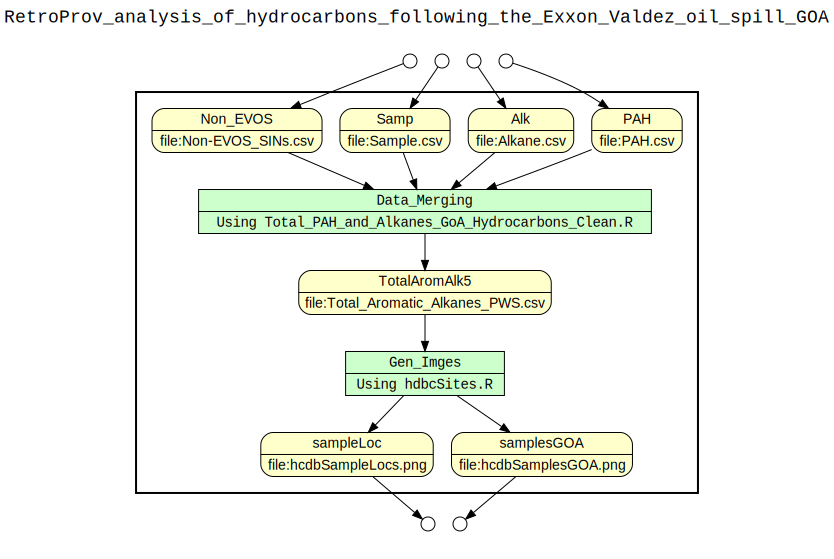
\includegraphics{./results/aoos_retro_wf_graph.pdf}


\end{document}
